\documentclass[10pt]{book}
\usepackage[utf8]{inputenc}
%\usepackage[T1]{fontenc}
\usepackage{tgbonum}
\usepackage[english]{babel}
\usepackage{graphicx}
\usepackage{amsmath}
\usepackage{amssymb}
\usepackage{hyperref}
\usepackage{epsf}
\usepackage{float}
\usepackage{mathpazo}
\usepackage
[
a4paper,% other options: a3paper, a5paper, etc
left=2.2cm,
right=2.2cm,
top=3cm,
bottom=3cm,
]{geometry}
%\geometry{hmargin=3.5cm, vmargin=2.5cm}
\usepackage{fancyhdr}
\pagestyle{fancy}
\fancyhf{}
\rfoot{\thepage}
\renewcommand{\headrulewidth}{0pt}
\usepackage{color}
\graphicspath{{DWGs/}}
\usepackage{graphicx}
\usepackage{wrapfig}
\usepackage{graphicx}
\usepackage{multicol}
\usepackage{enumitem}
\usepackage{xcolor}
\usepackage{framed}
\definecolor{shadecolor}{RGB}{139, 231, 3}
\usepackage{epigraph}

\usepackage{tcolorbox}
\definecolor{mycolor}{rgb}{0.122, 0.435, 0.698}

\newtcbox{\mb}{nobeforeafter,colframe=mycolor,colback=mycolor!10!white,boxrule=0.5pt,arc=4pt,
  boxsep=0pt,left=6pt,right=6pt,top=3pt,bottom=3pt,tcbox raise base}

\usepackage{eso-pic}
\newcommand\BackgroundPic{%
\put(-50,-0){%
\parbox[b][\paperheight]{\paperwidth}{%
\vfill
\centering
\includegraphics[height=\paperheight,%
keepaspectratio]{DWGs/cover.png}%
\vfill
}}}

\usepackage{anyfontsize}
\usepackage{t1enc}

% CHAPTER STYLE =================================================

\makeatletter
\def\thickhrulefill{\leavevmode \leaders \hrule height 1ex \hfill \kern \z@}
\def\@makechapterhead#1{%
  \vspace*{10\p@}%
  {\parindent \z@ \raggedleft \reset@font
            \scshape \@chapapp{} \thechapter
        \par\nobreak
        \interlinepenalty\@M
    \Huge \bfseries #1\par\nobreak
    %\vspace*{1\p@}%
    %\hrulefill
    \par\nobreak
    \vskip 100\p@
  }}
\def\@makeschapterhead#1{%
  \vspace*{10\p@}%
  {\parindent \z@ \raggedleft \reset@font
            \scshape \vphantom{\@chapapp{} \thechapter}
        \par\nobreak
        \interlinepenalty\@M
    \Huge \bfseries #1\par\nobreak
    %\vspace*{1\p@}%
    %\hrulefill
    \par\nobreak
    \vskip 100\p@
  }}

\begin{document}

% TITLE PAGE ====================================================

\begin{titlepage}
\AddToShipoutPicture*{\BackgroundPic}
\ \\[4cm]
{\sffamily \color{white}
\begin{center}
\fontsize{66}{10}\selectfont \fontfamily{qcr}\selectfont Fluid  Toolbox
\end{center}
}
\vfill
{\fontsize{20}{20}\color{white}\sffamily Science Docs \hfill\color{white} Kamila Zdybał}
\end{titlepage}


% EX LIBRIS PAGE ================================================

\thispagestyle{empty}
\begin{center}
\vspace*{4cm}
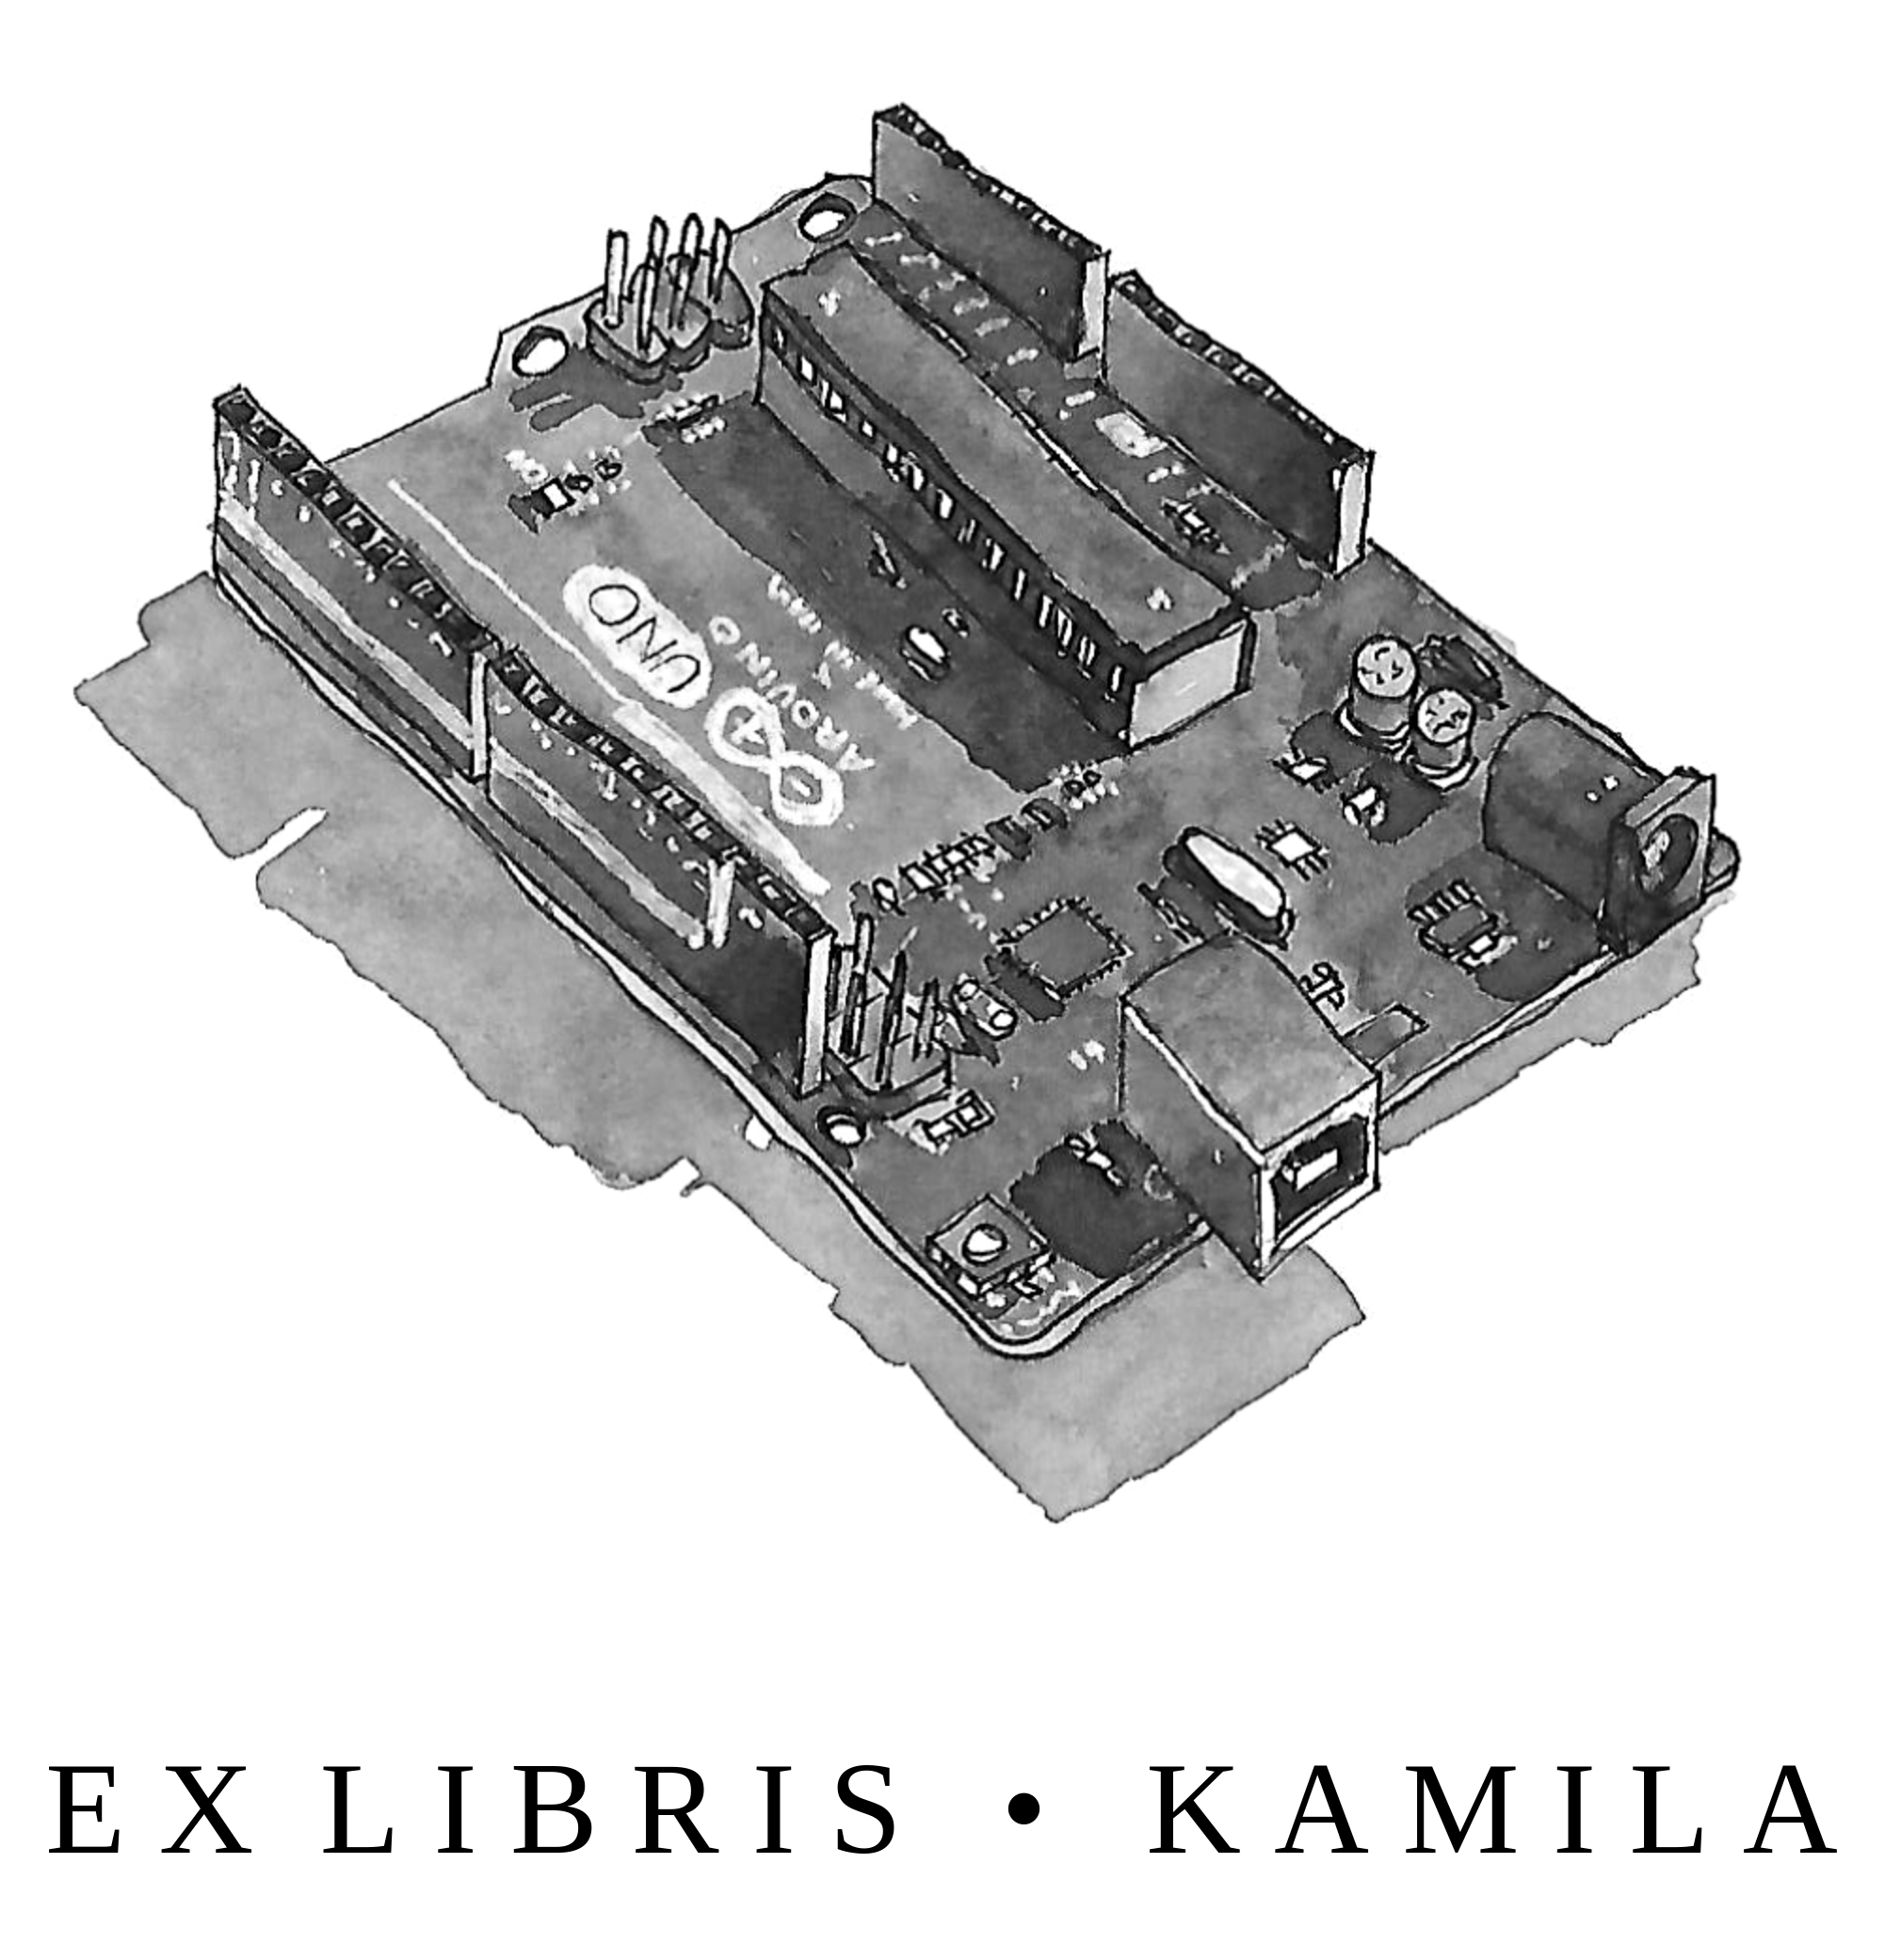
\includegraphics[width = 80mm]{ex_libris_arduino.png}

\vspace*{2cm}

Copyright \textcopyright \, K. Zdybał, 2018

For more projects similar to this one

visit me on GitHub: \verb|@camillejr|

\verb|camillejr.github.io/science-docs/|

To contact me personally drop me a line at:

\verb|kamilazdybal@gmail.com|

\vspace*{2cm}

\verb|Fluid Toolbox|

\verb|version 1.0|

Typeset with \LaTeX

\vspace*{1.8cm}

\noindent This work is licensed under the Creative Commons

Attribution-NonCommercial-ShareAlike 4.0 International 

(CC BY-NC-SA
4.0) license.
\end{center}



\setlength{\parskip}{0.6em}
\setlength{\parindent}{0cm}

\tableofcontents

\chapter*{Preface}
\chaptermark{Preface}
% Fluid Toolbox content

\rightline{{\rm \textit{"Use it well."}}}

\rightline{{\rm --- Prof. Dumbledore}}

\textbf{Fluid Toolbox} is a collection of human-readable, pseudo-random study notes. It contains descriptions and explanations of fluid dynamics, fluid mechanics and aerodynamics related concepts, presented in a way that resembles the record of my understanding of them. It is meant to be used complimentary to the regular textbook, since it may provide additional insight but it will not substitute a mathematical rigor nor thoroughness of a standard course in the subject. I believe that working side by side with a course it can become indeed a useful toolbox of concepts that are ready to understand and use in your personal projects.

\chapter{Differentiation}

Differentiation is a way to make discrete things continuous.

\chapter{Drag force}

The mathematical description of the drag force begins with making a guess. It is an intuitive guess which answers the question: what physical quantities affect the value of the drag force on an object moving through a fluid? The thought process done on this question gives the following four quantities:

relative fluid-object velocity $\upsilon$ \,\,\,\,\,\,\,\,\,\,\,\,\,\,\,  fluid density $\rho$ \,\,\,\,\,\,\,\,\,\,\,\,\,\,\, fluid viscosity $\mu$ \,\,\,\,\,\,\,\,\,\,\,\,\,\,\, geometry of an object $D$

We assume that the drag force is a combination of these quantities to some yet unknown powers and we use dimensional analysis to find those powers.

\begin{equation}
F_D = \upsilon^a \rho^b \mu^c D^d
\label{eq:drag_force}
\end{equation}

Writing out the units of the above equation we get:

\begin{equation*}
\Big[ \frac{kg \cdot m}{s^2} \Big] = \Big[ \frac{m}{s} \Big]^a \cdot \Big[ \frac{kg}{m^3} \Big]^b \cdot \Big[ \frac{kg}{m \cdot s} \Big]^c \cdot \Big[ m \Big]^d
\end{equation*}

Shuffling around a bit:

\begin{equation*}
kg \cdot m \cdot s^{-2} = kg^{b+c} \cdot m^{a -3b - c + d} \cdot s^{-a - c}
\end{equation*}

Hence:

$1 = b+c$

$1 = a - 3b - c + d$

$-2 = - a - c$

The simple fact that this set of equations cannot be solved exactly (there is four  uknown powers and only three equations) is going to call experiment for help, which you will notice in the next few passages.

Let's then write the set of equations by means of one of the unknowns $c$:

$a = 2 - c$

$b = 1 - c$

$d = 2 - c$

\newpage

Subsituting back to the equation \ref{eq:drag_force} we get:

\begin{equation}
F_D = \upsilon^{2 - c} \rho^{1 - c} \mu^c D^{2 - c} 
\label{eq:drag_force_powers}
\end{equation}

Structuring the equation still a bit gives:

\begin{equation}
F_D = \upsilon^2 \rho D^2 \cdot \Big[ \frac{\upsilon \rho D}{\mu} \Big]^{-c}
\label{eq:drag_force_powers}
\end{equation}

It always feels comfortable to find the Reynolds number in your equation, so there it is:

\begin{equation}
F_D = \upsilon^2 \rho D^2 Re^{-c}
\label{eq:drag_force_powers}
\end{equation}

We get finally that the drag force is proportional to some unknown power of the Reynolds number.


In fact, we will not leave it there yet, since there is an interesting last point to say. Instead of the above equation, we will say that the drag force is proportional to some unknown function $C_D$ of the Reynolds number. We also recognise that we may rewrite the quantity $\upsilon^2 \rho$ as the dynamic pressure $\frac{\upsilon^2 \rho}{2}$, since multiplying the right hand side by $\frac{1}{2}$ will not spoil the dimensional equality of both sides. The quantity $D^2$ has got the unit of area, so we exchange it for the quantity $A_{\perp}$, representing the frontal area of an object. The equation for the drag force becomes:

\begin{equation}
F_D = \frac{\upsilon^2 \rho}{2} A_{\perp} C_D (Re)
\label{eq:drag_force_powers}
\end{equation}

The unknown function $C_D (Re)$ is called the \textbf{drag coefficient}. That is where we call for experiment.

Questions:

What would have happened if we wrote the powers in terms of some power other than $c$?












\chapter{Circulation}



Circulation is defined as:

\begin{equation}
\Gamma = \oint_C \vec{\upsilon} \cdot \vec{dl}
\end{equation}

The dot operation gives a scalar which is expressing "how much" in the direction of the other vector is this vector.

\begin{figure}[H]
\centering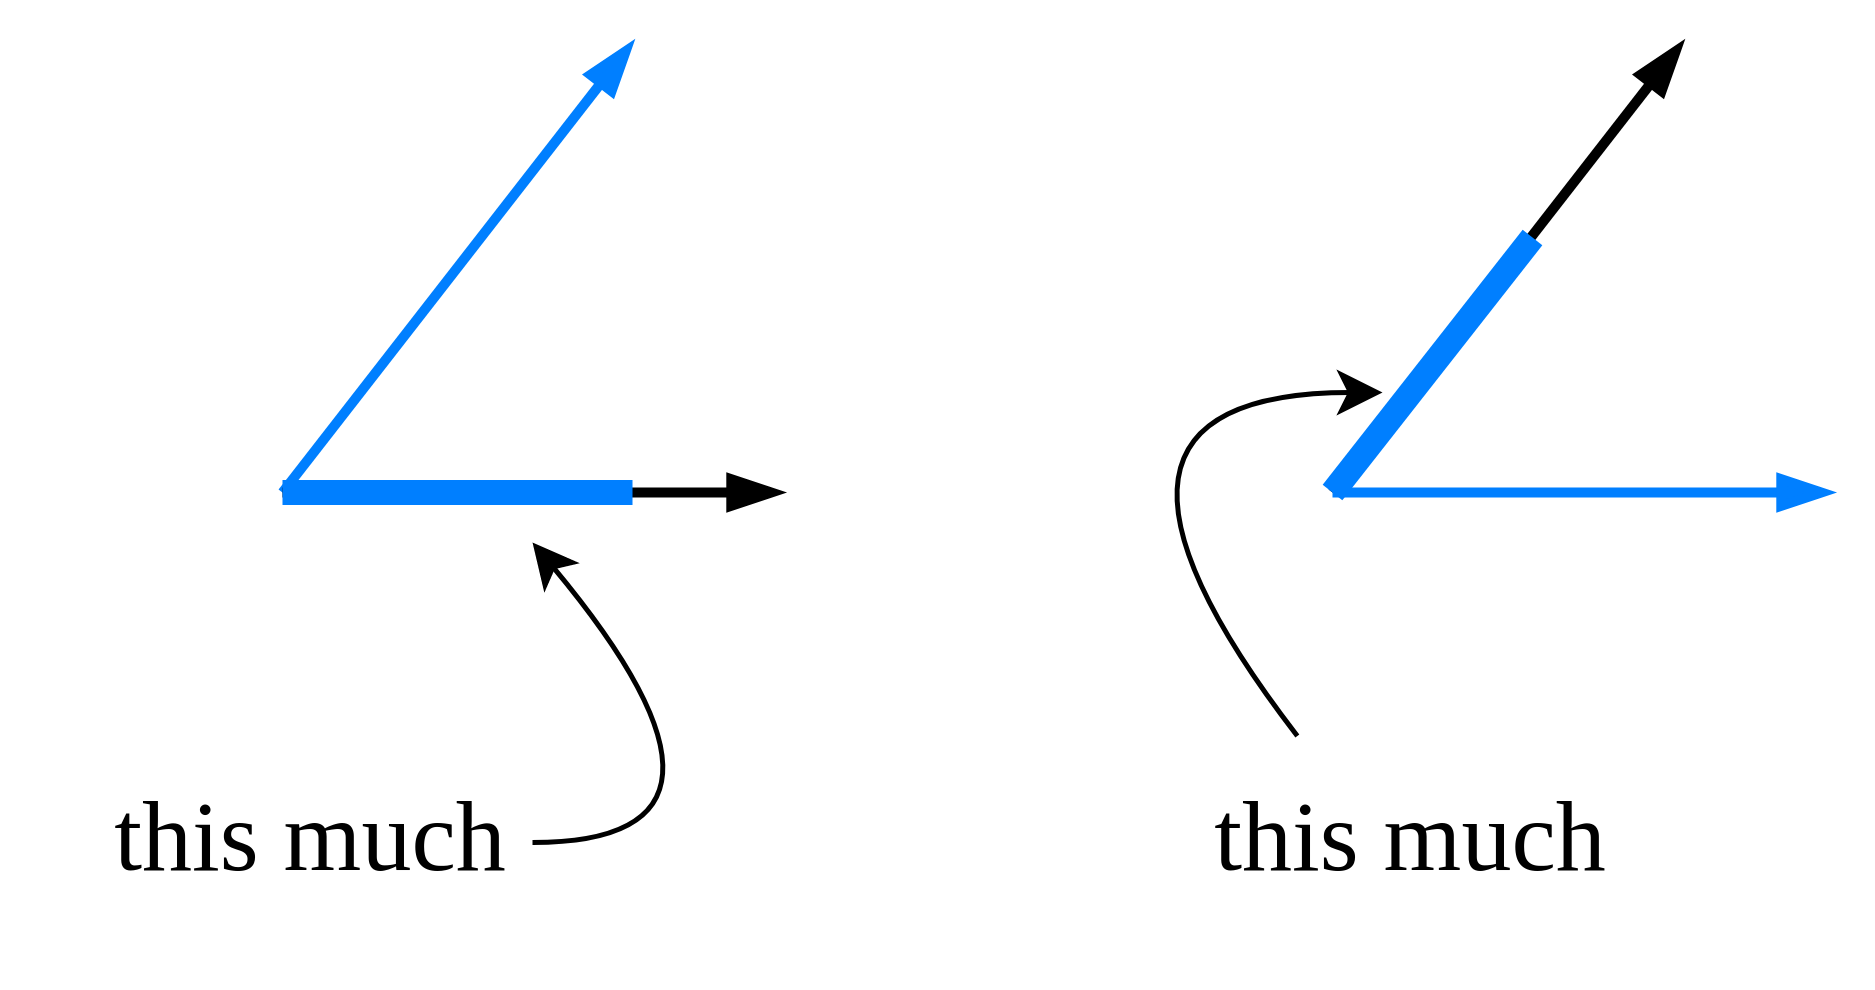
\includegraphics[width=5cm]{circulation_dot_prod}
\caption{Dot product of two vectors.}			
\label{fig:learning_curve}
\end{figure}

When they are $\perp$, the dot product is zero.

In the concept of circulation, you ask "how much" at any point on the curve $C$ the velocity vector at that point is in the direction of the curve's geometry. Now, that doesn't yet sound as something to do with "circulating". For the moment, I would think that it's more of an "on-trackness". Something, that in real world would be for instance the measure of how much the vehicle's velocity is in the direction of the road geometry.

But then you realise an important detail of "$\circ$" on the integral symbol, which means that the curve should be a closed curve - a loop.

When you perform integration, which means summing up every little $\vec{\upsilon} \cdot \vec{dl}$ as you go around the loop, you count "how much" at every point on the loop, the velocity vector at these points is in the direction of the loop's geometry (at these points).

If we were to place a small particle at some starting point $P$ on the loop, the circulation would tell us "how much" the velocity field which this particle is subjected to, is tending to move that particle around the loop.

It can be very intuitive when you take a look at these two pictures:



It's no surprise that when the velocity is everywhere perpendicular to the loop's geometry, the circulation around the loop is zero. If you were to place a particle at any point on the loop, such velocity field would act to immediately displace the particle off the loop. Therefore, the particle would have no way of "circulating" around the loop.

On the other extreme is the case when the velocity field is everywhere tangent to the loop's geometry. Anywhere the particle goes on the loop, the velocity at that point would act to keep the particle moving around the loop.

Questions:

\begin{enumerate}
\item Why closed loop? Would it have any meaning if we calculated circulation along any general spline?

\item How to chose loops so that the circulation we calculate is of the most meaning to us?

\item What does the zero, positive, negative circulation mean?

\item Can circulation be infinite?
\end{enumerate}



\chapter{Vorticity}


\begin{enumerate}
\item Why is vorticity concept needed? Isn't it something kind of like circulation?

\end{enumerate}


\chapter{Stoke's theorem}






\chapter{Material derivative}

\chapter{Gauss's law}

\chapter{On the road to the Navier-Stokes equations}

\chapter*{Appendix}

\newpage
\thispagestyle{empty}

\chapter*{About the author}

I am a recent graduate in civil engineering and a long-time passionate of the fluid business. My journey through fluid mechanics has begun during my first visit in a wind tunnel laboratory, where my future supervising Professor winked at me when encouraging students to join his research. Since then I wrote two theses under his guard: my Bachelor thesis on the subject of small-scale wind turbines and my Master thesis on the wind action causing flutter of bridges.

In the meantime I worked in a wind engineering company in the UK, where I had a chance to take part in every step of wind tunnel testing of tall buildings, occasionally even gluing some model details.

I was also a stagiaire at the von Karman Institute for Fluid Dynamics in Belgium, where apart from falling in love with French and Dutch languages, I studied data decomposition methods in linear algebra and applied them to approximate fluid flow phenomena.

I am now waiting for my next destination in this journey.



\begin{flushright}

%\ \\[6cm]

\includegraphics[width = 100mm]{cover.png}

\setlength{\parskip}{0.1em}
\setlength{\parindent}{0cm}
\ \\[0.5cm]
\textit{The cover photo:} Whenever the weather permits I enjoy exploring distant places with my bicycle. 

This photo is a view from the coast of the Cres island in Croatia, October 2016.
\ \\[0.1cm]
Photo by: J. Aleksanderek
\end{flushright}




\begin{thebibliography}{50}
\thispagestyle{empty}
\end{thebibliography}



\end{document}